\section{Introduction}\label{sec_introduction}

Hard parameter sharing (HPS) for multi-task learning is widely used in empirical research and goes back to the seminal work of \cite{C97}.
Recent work has revived interests in this approach because it improves performance and reduces the cost of collecting labeled data \cite{R17}.
It is generally applied by sharing the feature layers between all tasks while keeping an output layer for every task.
Often, hard parameter sharing offers two critical advantages if successfully applied.
First, it reduces model parameters since all tasks use the same feature space.
Second, it reduces the amount of labeled data needed from each task by augmenting the entire training dataset.

Hard parameter sharing works as an inductive transfer mechanism and a regularizer that reduces overfitting, both of which have great intuitive appeal \cite{R17}.
For example, by restricting the shared space's size, HPS encourages information sharing among multiple tasks \cite{KD12}.
Another source of inductive bias comes from the tasks and depends on datasets' properties such as sample sizes and task covariances \cite{WZR20}.
However, how these dataset properties impact HPS has not been well established.
%It becomes increasingly important to understand HPS' formal generalization properties.
Part of the challenge may be that HPS' generalization performance depends intricately on the sample size ratios and covariate shifts between tasks, and is not amenable to standard concentration results.
Previous results based on Rademacher complexity or VC dimensions have considered cases where all tasks' sample sizes are equal to logarithmic factors of the feature dimension \cite{B00,MPR16}, and when all tasks' sample sizes increase simultaneously \cite{AZ05,M06}.
%For, the generalization error scales down as the sample sizes of all tasks increase, when applied to the multi-task setting \cite{B00,AZ05,M06,MPR16,WZR20}.

\begin{figure*}[!t]
	\begin{subfigure}[t]{0.5\textwidth}
		\centering
		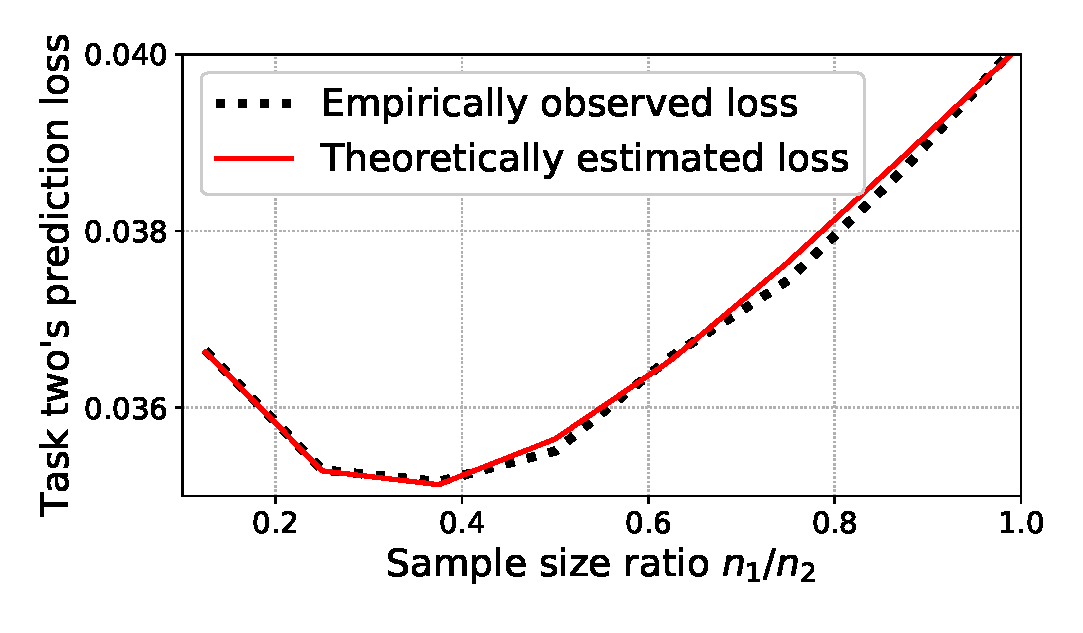
\includegraphics[width=0.745\textwidth,valign=t]{figures/sample_ratio_c2_400.eps}
		\caption{Covariate shift}
		\label{fig_intro_arch}
	\end{subfigure}\hfill
	\begin{subfigure}[t]{0.5\textwidth}
		\centering
		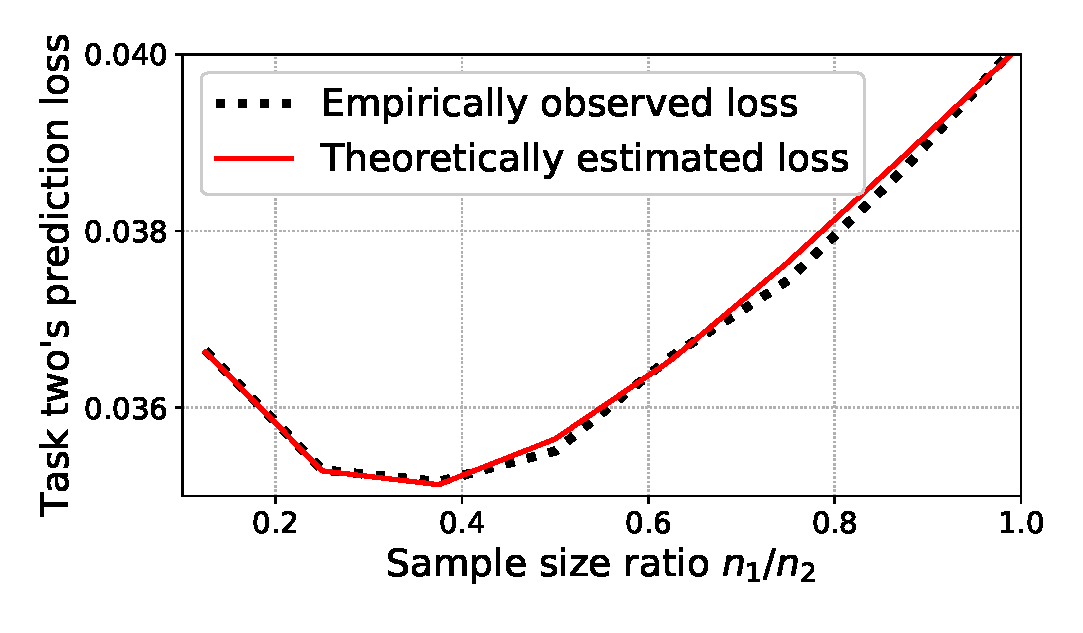
\includegraphics[width=0.745\textwidth,valign=t]{figures/sample_ratio_c2_400.eps}
		\caption{Varying sample size ratio}
		\label{fig_intro_sample_size_b}
	\end{subfigure}
	\vspace{-0.1in}
	\caption{
	Left: an illustrative picture of HPS.
	Right: an illustrative example of using HPS for two tasks $X_1, Y_1$ and $X_2, Y_2$ with sample size $n_1, n_2$, respectively.
	Increasing $n_1/n_2$ decreases task two's prediction loss initially but increase afterward. This phenomenon occurs due to different bias-variance tradeoffs as $n_1/n_2$ increases. Our result provides an estimated loss (solid line) that accurately matches the empirical loss (dotted line).
	See Section \ref{sec_simulation} for the precise setting.}
	\label{fig_intro_sample_size}
\end{figure*}



This paper presents new techniques to study hard parameter sharing and establishes a number of new results.
We consider regression analysis, which is arguably one of the most fundamental problems in statistics and machine learning.
We are interested in the \textit{high-dimensional} setting, where each dataset's sample size and feature dimension grow linearly instead of logarithmically.
This setting captures the fact that a single task's sample size is usually insufficient for accurate learning in many applications.
For example, if a dataset's sample size is only a constant factor of dimension in linear regression, the variance is also constant (cf. Fact \ref{fact_tr}).
The high-dimensional setting is challenging but is crucial for understanding how datasets' sample sizes impact generalization performance.




%\subsection{Summary of Results}

Our first result (Theorem \ref{thm_many_tasks}) applies to multi-label prediction settings where all datasets have the same features (and sample size), and we want to make several predictions for every input (cf. examples in \cite{hsu2009multi}).
We analyze the global minimizer of $f(A, B)$, and provide a sharp bias-variance decomposition of its (out-of-sample) prediction loss for any task.
This setting is tractable even though in general, $f(A, B)$ is non-convex in $A$ and $B$ (e.g. matrix completion is a special case for suitably designed $X^{(i)}, Y^{(i)}$).
%We show that the prediction loss of HPS admits a clean bias-variance decomposition.
Our result implies that when all tasks have the same features but different labels, for any task, HPS helps reduce the task's variance compared to single-task learning but increases bias.

Our second result (Theorem \ref{thm_main_RMT}) applies to two tasks with arbitrarily different sample size ratios and covariate shifts.
While we can no longer characterize $f(A, B)$'s global minimum because of non-convexity, we can still provide a sharp bias-variance tradeoff of any local minimizer's prediction loss for both tasks.
Despite being a simple setting, we observe several non-trivial phenomena by varying sample size ratios and covariate shifts between the two tasks.
See Figure \ref{fig_intro_sample_size_b} for an illustration of the former.
Consequently, using our precise loss estimates, we observe several qualitative properties of HPS for varying dataset properties.
\begin{itemize}
	\item \textit{Sample efficiency (Example \ref{ex_same_cov})}:
	One advantage of combining multiple datasets is that the requirement for labeled data reduces compared to single-task learning, a phenomenon that \cite{ZSSGM18} has observed empirically.
	Our results further imply that HPS's sample efficiency depends on model-specific variances across tasks vs. the noise variance and is generally high when the latter is large.

	\item \textit{Sample size ratio (Example \ref{ex_sample_ratio})}: Increasing one task's sample size does not always reduce another task's loss. In a simplified setting, we find that the task loss either decreases first before increasing afterward or decreases monotonically depending on how fast the bias grows. These two trends result from different bias-variance tradeoffs. This result is surprising because previous generalization bounds in multi-task learning typically scale down as all tasks' sample sizes increase, thus do not apply for different sample size ratios.

	\item \textit{Covariate shift (Example \ref{ex_covshift})}: In addition to sample sizes, variance also scales with two datasets' covariate shifts. For a large sample size ratio, HPS's  variance is smallest when there is no covariate shift. Counterintuitively, for a small sample size ratio, having covariate shifts reduces variance through a complementary spectrum. We achieve this result through a novel characterization on the inverse of the sum of two sample covariance matrices with arbitrary covariate shifts. See our discussion of proof techniques below for details.
\end{itemize}


Finally, we discuss the practical implications of our work.
Our sample size ratio study implies a concrete progressive training procedure that gradually adds more data until performance drops.
For example, in the setting of Figure \ref{fig_intro_sample_size_b}, this procedure will stop right at the minimum of the local basin.
We conduct further studies of this procedure on six text classification datasets and observe that it reduces the computational cost by $65\%$ compared to a standard round-robin training procedure while keeping the average accuracy of all tasks simultaneously.

%\medskip
%\noindent\textbf{Proof techniques.}
%There are two main ideas in our analysis. The proof of our first result uses a geometric intuition that hard parameter sharing finds a ``rank-$r$'' approximation of the datasets.
%We carefully keep track of the concentration error between the global minimizer of $f(A, B)$ and its population version (cf. equation \eqref{eq_A_star}).
%The proof of our second result is significantly more involved because of different sample sizes and covariate shifts. We show that the inverse of the sum of two sample covariance matrices with arbitrary covariate shifts converges to a deterministic diagonal matrix asymptotically (cf. Theorem \ref{thm_main_RMT}).
%We use recently developed techniques from random matrix theory to show a sharp convergence rate.
% to obtain a sharp estimate on the..., which is commonly referred to as the \emph{local law}.
%\HZ{add several sentences on the technical insight}
%One limitation of our analysis is that in Example \ref{ex_sample_ratio}, there is an error term that can result in vacuous bounds for very small $n_1$ (cf. equation \eqref{cor_MTL_error}).
%We believe our result has provided significant initial insights, and it is an interesting question to tighten our result.
%See Section \ref{sec_conclude} for more discussions of the technical challenge.





%\paragraph{Organizations.}
The rest of this paper is organized as follows.
In Section \ref{sec_same}, we present the bias-variance decomposition for hard parameter sharing.
In Section \ref{sec_diff}, we describe how varying sample sizes and covariate shifts impact hard parameter sharing using random matrix theory.
In Sections \ref{sec_simulation}, we validate our results in simulations.
In Section \ref{sec_conclude}, we summarize our work and discuss future work.
Section \ref{sec_text} describes our study on text classification tasks.
Section \ref{app_proof_error_same_cov}, \ref{appendix RMT}, and \ref{app_iso_cov} present proofs of our results.
